\documentclass[11pt,a4paper]{report}

\usepackage[utf8]{inputenc}
\usepackage[T1]{fontenc}

\pagestyle{empty}

\usepackage{graphicx} % Include figure files
\usepackage{amstext,amsbsy,amssymb}
%\usepackage{times} 

%% Numbered problems
\newcounter{excount}[chapter]
\newenvironment{exercise}[1][]{\addtocounter{excount}{1} \noindent {\bf Problem
    \arabic{excount} \ \ #1}\hspace{2mm}}{\vspace{4mm}}


\title{FYS3120 Classical Mechanics and Electrodynamics\\ 
\vspace{15mm}Problem set 4}


%%%%%%%
\begin{document}
%%%%%%%
\maketitle


%%%%%%%%
\begin{exercise}
The figure shows a rod of length $b$ and mass $m$, with the mass evenly distributed along the rod.
One endpoint of the rod is constrained to move along a horisontal line and the other endpoint along a vertical line. The two lines are in the same plane. There is no friction and the acceleration due to gravity is $g$. The set-up is illustrated in Fig.~\ref{fig:con_rod}.

%%%%%%%%%%
\begin{figure}[h]
\begin{center}
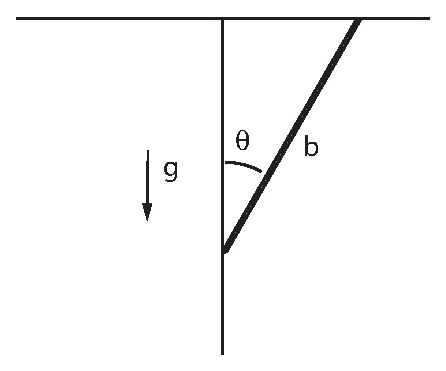
\includegraphics[width=5cm]{ConstrainedRod.eps}
\end{center}
\caption{Constrained rod.}
\label{fig:con_rod}
\end{figure}
%%%%%%%%%% 

\begin{itemize}
\item[\bf a)] Find the Lagrangian $L$ with the angle $\theta$ as coordinate, and show that Lagrange's equation gives
\begin{equation}
\ddot\theta+{3g\over {2b}}\sin\theta=0.
\end{equation}
{\it Hint:} For the moment of inertia of the rod, see Problem 2 in Set 2.
\item[\bf b)] What is the stable equilibrium position of the rod? Find the period $T_0$ for small oscillations about equilibrium.
\item[\bf c)] Since $L$ has no explicit time dependence, there is a corresponding constant of motion. What is the expression for this constant and what is the physical interpretation? Comment on how the expression is related to the equation of motion.
\item[\bf d)] Assume the rod oscillates about the equilibrium position with a maximum angle $\theta_0$, with $0<\theta_0\leq \pi/2$. Show that the period $T$ of the oscillations is generally expressed by the integral
\begin{equation}
T=T_0 {\sqrt 2\over \pi} \int_0^{\theta_0}\frac{d\theta}{\sqrt{\cos\theta-\cos\theta_0}}.
\end{equation}
Determine the ratio $T/T_0$ for the maximum amplitude $\theta_0=\pi/2$. {\it Hint:} In Rottman you will find a general formula, which can be used to express the integral in terms of the Euler gamma-functions. Give the numerical value of the ratio.
\end{itemize}
\end{exercise}

%%%%%%%%
\begin{exercise}[Reduced mass\\]
Let us look at the generic two-body problem with two objects of mass $m_1$ and $m_2$. Assume that the potential is only dependent on the distance between the two objects, as would be the case for both gravitational and electrostatic potentials.

\begin{itemize}
\item[\bf a)] Write down the Lagrangian $L$ in terms if the coordinates ${\vec r}_1$ and ${\vec r}_2$ of the two objects.
\item[\bf b)] Make the change of variables to the coordinates $(\vec r, \vec R)$, where
\begin{eqnarray}
{\vec r} &=& {\vec r}_1 -{\vec r}_2,\\
{\vec R} &=& \frac{m_1}{m_1+ m_2}{\vec r}_1 + \frac{m_2}{m_1+ m_2}{\vec r}_2,
\end{eqnarray}
and show that the resulting Lagrangian is
\begin{equation}
L= \frac{1}{2}(m_1+m_2)\dot{\vec R}^2+ \frac{1}{2}\mu\dot{\vec r}^2-V(r),
\end{equation}
where
\begin{equation}
\mu=\frac{m_1m_2}{m_1+ m_2},
\end{equation}
is the {\bf reduced mass}.
\item[\bf c)] Find Lagrange's equations in the new coordinates and solve for the motion of $\vec R$.
\item[\bf d)]  What is the physical interpretation of these new coordinates and the change of variables in the Lagrangian?
\end{itemize}


\end{exercise}




\end{document}
